
 
  \chapter{Implementação web} \label{CHP:RAILS}%%
            Conforme citado no capítulo dois, utilizaremos o framework web chamado Ruby on Rails, implementado sobre a linguagem Rails.
    \section{Ambientação}
     
    Para a configuração do ambiente Ruby on Rails, foram utilizadas as soluções de \cite{railsinstaller}, que implementou facilitadores para instalação em ambientes Windows e OS X. Porém, os aplicativos necessários podem ser instalados separadamente. Os necessários para a nossa aplicação foram:
\begin{itemize}
\item Ruby 1.9.3 -Interpretador da linguagem Ruby
\item Rails 3.2.11 - Pacote contendo todo o framework Rails utilizado
\item Git 1.7.10 - Controlador de versão Git. Utilizamos para o controle da versão junto ao GitHub e para fazer o deploy no Heroku
\item RVM1.16.17 - Gerenciador de versões Ruby
\item Bundler 1.2.1 - Controle de dependências (Gems\footnote{Gems sã pacotes que contém todoa informação de arquivos a serem insalados.})
\end{itemize}     
    Uma das decisões mais importantes no processo de manufatura de uma aplicação é a escolha da ferramenta ideal de desenvolvimento, que forneça agilidade e os recursos necessários para o desenvolvedor.
	
    Por ser uma aplicação em Ruby, onde os arquivos de código e de configuração são baseados em texto puro, o Ruby on Rails não exige nenhuma ferramenta avançada de criação.     Em outras palavras, utilizar um editor de texto simples ou uma \ac{IDE} é uma decisão pessoal.
	
    As IDE's mais comuns para se trabalhar com Rails são:
\begin{itemize}
\item RubyMine - Intellij IDEA
\item Aptana Studio 3 - antes conhecida como RadRails, plugin para Eclipse
\item Ruby in Steel- Visual Studio
\item NetBeans - (até a versão 6.9)
\end{itemize}     
    De acordo com \cite{caelum}, a maioria dos desenvolvedores Ruby on Rails não utiliza nenhuma \ac{IDE}, apenas um bom editor de texto e um terminal (ou prompt) de comando aberto.  Algumas ferramentas de texto boas para esse propósito, junto aos sistemas operacionais que suportam, são as seguintes:
\begin{itemize}
\item TextMate -  Mac OS X
\item Sublime Text - Mac OS X, Linux, Windows
\item Gedit - Mac OS X, Linux
\item Notepad++ - Windows
\item VI/Vim - Mac OS X, Linux, Windows
\end{itemize}
    Nesse projeto foi utilizado o TextMate, no ambiente Mac OS X.
    \section{Criação de aplicação}
            Uma vez que o Rails tenha sido instalado corretamente e, automaticamente, definido como variável de ambiente no terminal, pode-se executar o comando ``rails'' para criação de aplicação e módulos.  Pode-se, também,  verificar a versão do rails através do comando:
			
\begin{lstlisting}
    $rails --version
\end{lstlisting}
           
    A versão utilizada nesse projeto é a 3.2.11, a última disponibilizada. A fim de criar a aplicação, utilizando o banco de dados Postgre, foi executado o seguinte comando:
	\begin{lstlisting}
    $rails new iQuizzer -d postgresql
    \end{lstlisting}   
    Ao executar a ultima linha, o rails criou um diretório com alguns arquivos, que serão vistos na próxima seção.
     
    \section{Estrutura}
           
     
            Um projeto rails tem uma estrutura básica composta das seguintes pastas:
\begin{itemize}
\item App: contém os arquivos específicos da aplicação. Conforme citado no capítulo 2, o rails utiliza o padrão \ac{MVC}, e dentro desse diretório a divisão é feita através dos sub-diretórios model, view e controller;
\item Config: configurações diversas da aplicação;
\item db: contém as migrações (alterações no banco de dados durante o processo de desenvolvimento), além de alguns outros arquivos relacionados ao banco de dados
\item doc: documentação do sistema
\item lib: bibliotecas
\item log: algumas informações de log
\item public: nessa pasta estão contidos todos os arquivos públicos que serão servidos pela WEB
\item test: utilizado para testar a aplicação, normalmente quando se usa \ac{TDD}\footnote{Desenvolvimento orientado a testes é uma técnica de desenvolvimento de software onde um caso de teste é escrito para cada funcionalidade a ser implementada. A implementação deve validar o teste e o código refatorado para padrões aceitaveis.}. Em nosso projeto, não será utilizado.
\item Tmp: arquivos temporários de sessão e cache
\item Vendor: projetos dependentes (terceiros)
\end{itemize}     
     
    \section{Banco de dados}
    \subsection{PostgreSQL}
            Banco de dados são coleções de informações que se relacionam de forma que crie um sentido. Seu objetivo principal é representar abstratamente uma parte do mundo real, conhecida como Universo de Discurso \cite{ufmsbd}. 
			
    Na aplicação, foi utilizado um banco de dados relacional chamado PostgreSQL. Lançado em 1995, está atualmente na versão 9.1.4, sobre a licença BSD\footnote{BSD foi criada pela Universidade de Berkeley e é conhecida por ser uma licença de pouca restrição quando comparada a GNU. Ela permite que o software distribuído sobre a licença seja incorporada a produtos proprietários.}.
	
    A opção pela escolha do PostgreSQL deve-se ao bom suporte do Heroku a este \ac{SGBD}. Entretanto, outros motivos poderiam ser colocados em prol dessa decisão, a saber:
\begin{itemize}
\item Independência de plataforma - roda nos principais sistemas operacionais
\item Leve, podendo ser rodado em desktops convencionais
\item Instalação simples
\item Gratuito
\end{itemize}
    \subsection{Modelos}
            Conforme o diagrama de classes citado no capítulo 3, a aplicação possui algumas entidade, onde entidade é uma tabela presente no banco de dados e um active record contido na pasta app/models.
			
            O Rails possui uma forma bem simples de criar modelos, através de um comando de criação. Seja, por exemplo, a entidade Usuario, tal que seus campos e tipos de campos sejam passados como parâmetros de um comando de criação de modelos:
			
\begin{lstlisting}
    $rails generate model Usuario nome:string sobrenome:string 
	apelido:string pontos_criador:float pontos_jogador:float 
	username:string senha:string
\end{lstlisting}
            A execução desse comando gera os seguintes arquivos:
\begin{itemize}
\item Um arquivo de migração de tabela, que cria a tabela usuário no banco de dados
\item Uma classe chamada usuario.rb,  dentro de app/models,  e estende de ActiveRecord
\item Arquivos de teste
\end{itemize}     
    Após a criação do modelo, pode ser rodado o seguinte comando:
	\begin{lstlisting}
    $rake db:migrate
     \end{lstlisting}
    Esse comando tem a função de executar todas as migrações, ou seja, de alterar os dados no banco de dados. Caso seja necessária a modificação de um campo dessa tabela, como por exemplo, ao criar uma associação, pode ser criado um novo arquivo migration especificamente para isso.
	
    \subsection{Relacionamentos}
     
            Ao ser analisado o diagrama de classes da aplicação na seção 3.x, pode-se verificar que existem relacionamentos entre as entidades apresentadas. Tais entidades representam relações entre tabelas do banco de dados, as quais devem ser implementadas na camada de modelo da aplicação.
			
            Para relacionar tais modelos, deve-se informar ao Rails o tipo de relacionamento existente. Isso é feito declarando o tipo de relacionamento entre modelos nos active records. Os tipos de relacionamentos tratados são:
			
\begin{itemize}
\item $Belongs\_to$: é utilizado quando um modelo tem como atributo o id de outro modelo (em um relacionamento um para muitos ou um para um).
\item $has\_many$: associação contrária ao $belongs\_to$; indica que um determinado modelo tem muitas instancias de outro modelo
\item $has\_one$: similar ao $has\_many$, porém com apenas uma instância (relacionamento um para um)
\item $has\_and\_belongs\_to\_many$: associação muitos para muitos
\end{itemize}     

    As declarações de relacionamento criam alguns métodos de acesso automaticamente. Observe o código abaixo, do modelo de quiz e do modelo de pergunta:
	
\begin{lstlisting}[language=Ruby]
    #-- classe Quiz
    class Quiz < ActiveRecord::Base
      	#modojogo: 1 - random, 2 - ordenate
    	attr_accessible :titulo, :perguntas_attributes, :modojogo,
		 :maxquestoes, :descricao, :usuario_id
     
    	 has_many :perguntas
    end
     
    #--classe Pergunta
    class Pergunta < ActiveRecord::Base
    	attr_accessible :conteudo, :respostas_attributes
     
    	belongs_to :quiz
    	has_many :respostas
    end
	
\end{lstlisting}

    Nesses modelos, foi definido que pergunta pertence a quis, e que um quiz possui várias perguntas. Tais definições criam métodos de acesso automaticamente, como:
	
\begin{lstlisting}   
	quiz.perguntas #retorna array de perguntas
	pergunta.quiz #retorna objeto Quiz
	
\end{lstlisting}     

    O Rails não verifica automaticamente se a relação declarada funciona. Porém, de acordo com o princípio ``convenção sobre configuração'', definido no capítulo 2, é esperado que existam chaves estrangeiras do tipo $<modelo>\_id$ nas tabelas que possuam relacionamentos do tipo $belongs\_to$. Para tanto, devemos criá-las nas tabelas do banco, utilizando um objeto migration.
	
            Para criar um objeto migration, entre quiz e perguntas, utilizou-se, por exemplo, o seguinte generate do rails:
\begin{lstlisting}[language=Ruby]			
    Srails generate migration AddColumnQuizIdPergunta
 \end{lstlisting}   
       
    Isso gerou um arquivo migration  com o nome correspondente a $``<data\_hora> add\_column\_quiz\_id\_pergunta''$, no diretório /db/migrate. Implementou-se, então, o migration com o campo id:
	
\begin{lstlisting}[language=Ruby]
    classAddColumnQuizIdPergunta< ActiveRecord::Migration
    	def up
    	    add_column :Perguntas, :quiz_id, :integer
    	end
     
    	def down
    	end
    end
 \end{lstlisting}    
 
    Ao executar o script de execução, $rake db:migrate$, será executado um SQL de criação da coluna no banco de dados. É recomendado que as alterações sofridas no banco de dados ao longo do projeto utilizem migration, uma vez que é possível registrar toda a seqüência de alterações no banco e reproduzi-las em outros ambientes.
     
     
    \section{Rotas e REST}
            As rotas no rails servem para transformar determinadas requisições \ac{URL} em chamadas para controles particulares.  Algumas dessas rotas, para recursos, são utilizadas para o desenvolvimento da aplicação utilizando \ac{REST}, em conformidade ao definido no capítulo 2.
			
            Aplicações em Rails são ditas RESTful, associando o o protocolo \ac{HTTP} às operações de \ac{CRUD}. Na aplicação, tem-se as seguintes operações disponíveis:
\begin{itemize}
\item \emph{Get}: retorna o valor ou representação do recurso - \emph{select}
\item \emph{Post}: criação de um novo recurso - \emph{insert}
\item \emph{Put}: altera o recurso - \emph{update}
\item \emph{Delete}: remove o recurso - \emph{delete}
\end{itemize}     
    Para acessar o recurso, definimos uma rota de recurso no arquivo routes.rb. Seja o modelo de quiz; define-se o seguinte recurso:
\begin{lstlisting}
    # routes.rb
    resources :quizzes
 \end{lstlisting}      
    Para esse recurso, o rails automaticamente cria sete rotas de acesso, a saber:
\begin{itemize}
\item GET /quizzes:controller => ' quizzes ', :action => 'index'
\item POST /quizzes:controller => ' quizzes ', :action => 'create'
\item GET /quizzes /new:controller => ' quizzes ', :action => 'new'
\item GET /quizzes /:id:controller => ' quizzes ', :action => 'show'
\item PUT /quizzes/:id:controller => 'quizzes ', :action => 'update'
\item DELETE /quizzes /:id:controller => ' quizzes ', :action => 'destroy'
\item GET /quizzes /:id/edit:controller => ' quizzes ', :action => 'edit'
\end{itemize}     
    Para todas as rotas criadas, o Rails também cria os helpers (view do \ac{MVC}):
\begin{itemize}
\item    $quizzes\_path         \# => "/quizzes "$
\item    $new\_quiz\_path      \# => "/quizzes /new"$
\item    $edit\_quiz\_path(3)  \# => "/quizzes /3/edit"$
\end{itemize}     
     
    Os resultados dos métodos invocados pelas rotas, por padrão, são em \ac{HTML}. Entretanto, existem facilitadores no Rails para que esse retorno seja em \ac{XML} ou \ac{JSON}. Além disso, podemos passar no corpo de um \ac{HTTP} uma entrada em \ac{XML}/\ac{JSON}, de modo a ser interpretada pelo controller.
	
            Na aplicação, toda a comunicação entre o Web Service (aplicação rails) e o cliente (aplicação mobile) é feita através de \ac{REST} utilizando \ac{JSON}. Isso é possível utilizando um Format, como no exemplo abaixo:
\begin{lstlisting}[language=Ruby]
    # GET /quizzes
      # GET /quizzes.json
    def index
        @quizzes = Quiz.all
    	respond_to do |format|
          format.html # index.html.erb
          format.json { render :json => @quizzes }
   	   end
    end
     
 \end{lstlisting} 
            O método index é responsável por retornar um array com todos os quizzes. Se a requisição vier por \ac{HTML}, ou seja, do próprio site, a resposta será em \ac{HTML}; caso contrario, a resposta será em \ac{JSON}. Dessa forma, percebemos que a forma como os dados são requisitados é que diferenciam a saída .
     
    \section{Autenticação}
            Conforme foi definido no capítulo 3, um dos requisitos não funcionais é a segurança, ou seja, o sistema deve ser capaz de garantir que os dados de cada usuário estejam protegidos.
			
            A autenticação de um usuário busca verificar a identidade digital do mesmo. A partir da autenticação, o sistema autoriza o acesso ou não a determinados recursos do sistema.
			
           Na aplicação, a autenticação é feita através de tokens. Tokens são chaves criptografadas que identificam uma sessão do usuário. Optamos por disponibiliza-los no momento que o usuário realiza o login. Uma vez que o navegador (ou o aplicativo móvel nativo) obtenha o token, o acesso é garantido até que esse token expire.
			
            A fim de reduzir o tempo de desenvolvimento, utilizou-se uma gem chamada Devise, para autenticação e gerência de contas. Essa gem possui doze módulos para gerencia de conta, dos quais foram utilizados os seguintes, com as funções de:
\begin{itemize}
\item Database authenticable: encripta e armazena uma senha no banco de dados para validar a autenticidade de um usuário enquanto está logado.
\item Token Authenticable: usuários permanecem logados enquanto uma token autenticada for valida
\item Registerable: permite ao usuário criar contas
\item Recoverable: gera uma nova senha para o usuário e o manda instruções para realterar sua senha
\item Rememberable: gerencia e limpa tokens para lembrar o usuário de um cookie já salvo
\item Trackable: guarda informações de acesso, como o numero de vezes que o usuário logou, o momento do último login e o endereço IP.
\item Validatable: Valida a conta através de email/password.
\end{itemize}   
  
    O Devise cria algumas telas (helpers) por padrão. As telas de confirmação, envio de email, gerência de contas, senha e sessão são geradas de maneira básica. As imagens seguintes mostram algumas dessas telas, com o layout modificado pelo bootstrap, que será abordado na próxima seção.
	 \begin{figure}[H]
	   % Requires \usepackage{graphicx}
	   \centering
	   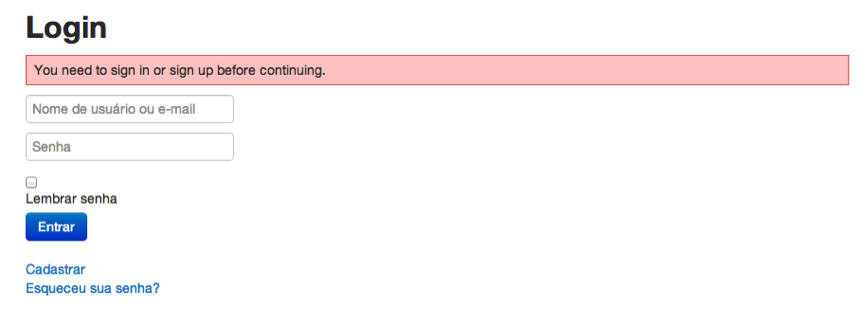
\includegraphics{figs/railslogin.png}\\
	   \caption{ Tela mostrada quando o usuario tenta acessar recurso e nao está logado }
	   \label{FIG:railslogin}
	 \end{figure}
	 
	 \begin{figure}[H]
	   % Requires \usepackage{graphicx}
	   \centering
	   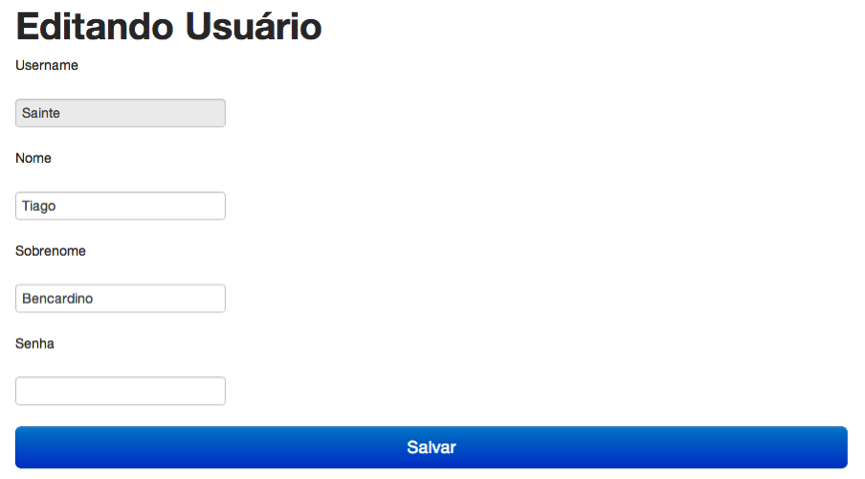
\includegraphics{figs/railsedituser.png}\\
	   \caption{ Edição de dados do usuário }
	   \label{FIG:railsuseredit}
	 \end{figure}
	 
	 \begin{figure}[H]
	   % Requires \usepackage{graphicx}
	   \centering
	   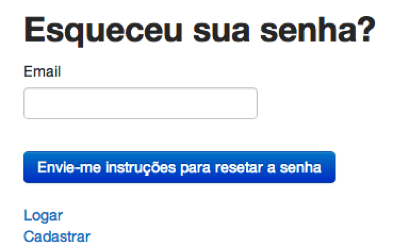
\includegraphics{figs/railsforgetpass.png}\\
	   \caption{ Lembrar senha do usuário }
	   \label{FIG:railsforgetpass}
	 \end{figure}

    Para a validação da sessão no mobile, utilizamos essencialmente manipulação por tokens. No momento que o usuário abre a aplicação, é verificado se o token é válido: caso não seja, uma tela pedindo nome de usuário e senha é mostrada. Após o usuário fornecer os dados, é enviada uma requisição em \ac{JSON} para \url{/api/v1/token_controller}, que verifica se os dados estão corretos e se o usuáriorealmente existe. Se tudo ocorrer corretamente, um token é retornado da requisição; caso contrario, uma mensagem contendo o erro é retornada.
	 \begin{figure}[H]
	   % Requires \usepackage{graphicx}
	   \centering
	   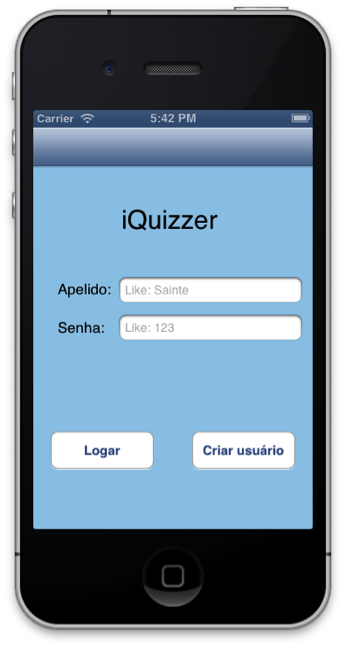
\includegraphics{figs/ioslogin.png}\\
	   \caption{ Login no mobile (iOS) }
	   \label{FIG:iOSlogin}
	 \end{figure}

    \section{Front-End}
            No modelo \ac{MVC}, a parte de view (visão) é responsável pelas interações com o usuário, recebendo as entradas e renderizando a saída. Os tipos de arquivos de fronteira mais comuns são o \ac{HTML}, ERB e o eRuby. Em nossa aplicação, utilizamos em quase todas as páginas a extensão ERB.
			
            Os controllers, por sua vez, são responsáveis por receber a ação de uma View e executar alguma lógica ligada a algum modelo. Basicamente, a função do controller é atender a requisições entre modelo e visão, fazendo toda a tradução necessária entre as camadas.
			
            Um controller pode ser criado através de um comando generate, como a seguir:
	\begin{lstlisting}
    $rails generate controller quizzes
    \end{lstlisting} 
            Esse comando irá criar uma classe chamada $quizzes_controller.rb$ e uma pasta chamada quizzes, dentro da pasta views. A ligação entre as camadas é feita automaticamente, devido ao conceito de ``convenção sobre configuração''.
			
            Nesse controller criado, foram colocados métodos de manipulação de dados (RESTful). Na parte de visão, colocamos alguns arquivos para manipular quizzes.  
			
            Veja, a seguir, o código da página index.html.erb. que tem como função listar quizzes e navegar para tela de criação:
\begin{lstlisting}[language=HTML]
<h1>Quizzes</h1>
     
<table class="table table-hover">
    <thead>
        <tr>
            <th>#</th>
            <th> Titulo </th>
            <th> Descricao </th>
            <th> Criador </th>
            <th> #Perguntas </th>
			</tr>
    </thead>
    <tbody>
	    <% @quizzes.each do |quiz| %>
            <tr>
                <td><%= quiz.id %></td>
                <td><%= link_to quiz.titulo, quiz %></td>
                <td><%= quiz.descricao %></td>
                <td><%= link_to quiz.user.username, quiz.user %></td>
                <td><%= quiz.perguntas.size %></td>
            </tr>
        <% end %>
    </tbody>
</table>
     
<%= link_to new_quiz_path do %>
    <button class="btn btn-large btn-block btn-primary" type="button">
        Criar quiz
    </button>
<% end %>
 \end{lstlisting} 
 
             Nesse código, é possível observar que existe código Ruby inserido entre os caracteres ``<\%'' e ``\%>''. Esses caracteres representam um escape do html para  o Ruby. Quando colocado com um sinal de igual, ``<\%='', o resultado da linha executada é impressa na tela final \ac{HTML} apresentada ao usuário.
			 
            É importante observar que todos os atributos de classe do controller, representados por um @, como em @quizzes, estão sobre o mesmo escopo.
			
    \subsection{Bootstrap}
            ``Elegante, intuitiva e poderoso framework de front-end para desenvolvimento web rápido e fácil'' - com essa descrição, o Bootstrap é apresentado em seu site oficial \cite{bootstrap}.  Lançado em Agosto de 2011 pelo Twitter, é atualmente o projeto mais popular do GitHub \cite{githubpop}.
			
            O Bootstrap é uma coleção livre de ferramentas para desenvolver sites e aplicações web. Basicamente, contém templates \ac{HTML}, JavaScript e \ac{CSS} para tipografia, formas, botões, gráficos, navegações, etc.
    Na aplicação, utilizamos o Bootstrap para personalização de botões, tabelas, divisão da página em duas seções e menu.
	 \begin{figure}[H]
	   % Requires \usepackage{graphicx}
	   \centering
	   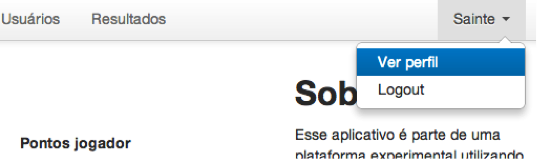
\includegraphics{figs/bootstrapcontrol.png}\\
	   \caption{ Exemplo de controle bootstrap }
	   \label{FIG:bootstrapcontrol}
	 \end{figure}
     
            Uma das funcionalidades mais aclamadas do Bootstrap é a adequação da tela para resoluções menores: quando colocado em telas de pouca largura, tipicamente em smartphones, a página se adequa para ser apresentada em um layout mais amigável para dispositivos móveis, como abaixo:
	 \begin{figure}[H]
	   % Requires \usepackage{graphicx}
	   \centering
	   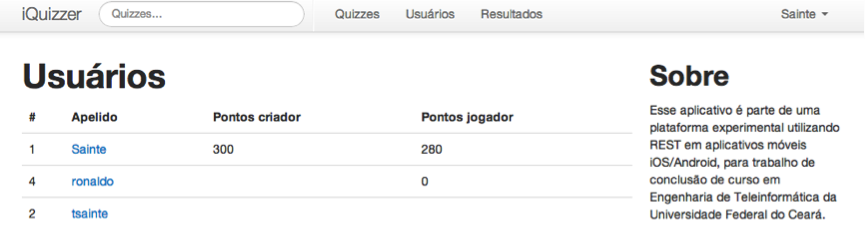
\includegraphics{figs/bootstraplayout1.png}\\
	   \caption{ Tela desktop extendida}
	   \label{FIG:bootstrapcontrol}
	 \end{figure}
	 
	 %%seria legal se ficassem lado a lado....
	 \begin{figure}[H]
	   % Requires \usepackage{graphicx}
	   \centering
	   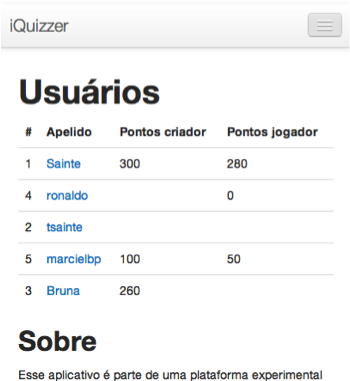
\includegraphics{figs/bootstraplayout2.png}\\
	   \caption{ Tela mobile com menu suprimido }
	   \label{FIG:bootstrapcontrol}
	 \end{figure}
	 \begin{figure}[H]
	   % Requires \usepackage{graphicx}
	   \centering
	   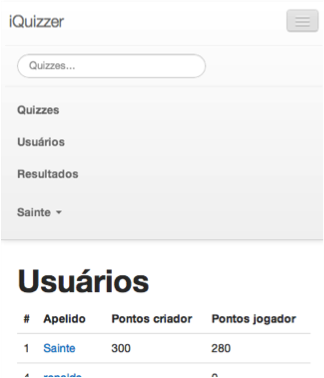
\includegraphics{figs/bootstraplayout3.png}\\
	   \caption{ Tela mobile com menu extendido }
	   \label{FIG:bootstrapcontrol}
	 \end{figure}

     
     
    \section{Deploy}
            Para que uma aplicação rails execute, é necessário um servidor de aplicação. Em ambiente de desenvolvimento, utilizamos o Webrick, que é um servidor já embutido em todas as aplicações. Para executá-lo, basta abrir o terminal, navegar até o diretório raiz da aplicação e executar o seguinte comando:
			
	\begin{lstlisting}		
    rails server
     \end{lstlisting}
	 
            Caso uma porta diferente da porta padrão seja necessária (3000), pode ser passado o parâmetro -p xxxx, onde xxxx é a porta desejada.
			
            O nosso ambiente de produção está hospedado como serviço no Heroku, sobre o runtime stack ``Celadon Cedar''. Para ativar, foi necessário fazer o cadastro, instalar o Heroku Toolbelt, efetuar login via terminal e fazer deploy. Mais detalhes podem ser encontrados no QuickStart do Heroku \cite{quickheroku}.
			
            A submissão de arquivos para o servidor do Heroku é feita através do controlador de versão Git. Para submeter, deve-se comitar o código e realizar um git push para o servidor. Caso seja necessário executar algum comando, como rake de migrations, usa-se o ``run'', conforme a seguir:
			
\begin{lstlisting}	
    heroku run rake db:migrate 
\end{lstlisting}